
% # COPYRIGHT:
%
%   Copyright (C)  2011 Jeremiah Mahler <jmmahler@gmail.com>.
%   Permission is granted to copy, distribute and/or modify this document
%   under the terms of the GNU Free Documentation License, Version 1.3
%   or any later version published by the Free Software Foundation;
%   with no Invariant Sections, no Front-Cover Texts, and no Back-Cover Texts.
%   A copy of the license is included in the file "fdl-1.3.txt".
%

\documentclass[12pt]{article}
%\documentclass[10pt]{article}

%\usepackage{mslapa}
\usepackage{hyperref}
\usepackage{amsmath}
\usepackage{graphicx}
\usepackage{ulem}
%\usepackage{vmargin}
\usepackage{tabularx}
\usepackage{sectsty}
\usepackage{pbox}
\usepackage{bigstrut}
\usepackage{enumerate}
\usepackage{parskip}  % add spaces between paragraphs
\input kvmacros  % Karnaugh Maps and Veitch charts
\usepackage[table]{xcolor}

%\usepackage{cleveref}

%\setpapersize{USletter}
\sectionfont{\normalsize}
\subsectionfont{\normalsize}

% configure \bigstrut size
% This configures spacing above and below rows in a tabularx.
%\renewcommand{\bigstrutjot}{6pt}
\renewcommand{\bigstrutjot}{2.0\jot}

\setlength{\parindent}{0in}

\raggedright

\begin{document}

% {{{ Cover Page

\centerline{\bf EECE 144}
\centerline{\bf Fall 2011}
\centerline{\bf}
\centerline{\bf Lab Report \#6}
\centerline{\bf Section 4}
\centerline{\bf 10/12/2011}

% signature area
\begin{center}
\begin{tabularx}{\textwidth}[b]{X l l}
Submitted by: Jeremiah Mahler & & \\
Signature & Printed Name & Date \\
\hline
\multicolumn{1}{|X|}{} & \multicolumn{1}{|l|}{\bigstrut \bf Jeremiah Mahler} & \multicolumn{1}{|l|}{\bf Oct 12, 2011} \\
\hline
\multicolumn{1}{|X|}{} & \multicolumn{1}{|l|}{\bigstrut \bf Marvanee Johnson} & \multicolumn{1}{|l|}{\bf Oct 12, 2011} \\
\hline
\end{tabularx}
\end{center}
% }}}

\section{Description/Objectives}

The objective of this lab is to simplify a function in to
two equivalent forms, one using NAND's and the other using NOR's,
then implement this in hardware.

\section{Procedure}
\label{sec:procedure}

The procedure for this lab consists of several parts.
First, using the given logic function, it is simplified
using Karnaugh Maps.
Then this simplified function is manipulated in to two
forms with one using only NAND's and the other using only NOR's.

The canonical SOP form of the equation used in this lab is
given in Equation \ref{eq:cansop}.

\begin{align}
f(a, b, c, d) &= \sum m(0, 2, 8, 10, 12, 13, 14, 15) \label{eq:cansop} \\
	    &= m_0 + m_2 + m_8 + m_{10} + m_{12} + m_{13} + m_{14} + m_{15}\notag \\
		&= a'b'c'd' + a'b'cd' + ab'c'd' + ab'cd' + abc'd' + abc'd + abcd' + abcd \notag
\end{align}

The truth table produced from Equation \ref{eq:cansop}
is shown in Figure \ref{fig:tt}.
And the Karnaugh Map produced from the truth table
is shown in Figure \ref{fig:karnmap}.
Using the groupings produced by the Karnaugh Map
results in the simplified form in Equation \ref{eq:simp}.

\begin{align}
f(a, b, c, d) &= ab + b'd' \label{eq:simp}
\end{align}

\begin{figure}[!hbt]
\begin{center}

\begin{tabular}{lr}
  \begin{tabular}[t]{r|cccc|c}
Index&$a$&$b$&$c$&$d$&$f$\\
\hline
0  &0&0&0&0 &1\\
1  &0&0&0&1 &0\\
2  &0&0&1&0 &1\\
3  &0&0&1&1 &0\\
4  &0&1&0&0 &0\\
5  &0&1&0&1 &0\\
6  &0&1&1&0 &0\\
7  &0&1&1&1 &0\\
8  &1&0&0&0 &1\\
9  &1&0&0&1 &0\\
10 &1&0&1&0 &1\\
11 &1&0&1&1 &0\\
12 &1&1&0&0 &1\\
13 &1&1&0&1 &1\\
14 &1&1&1&0 &1\\
15 &1&1&1&1 &1\\

  \end{tabular}
\end{tabular}
\end{center}

\caption{Truth table of Equation \ref{eq:cansop}.}
\label{fig:tt}
\end{figure}

\begin{figure}[!hbt]
\begin{center}

%\begin{tabular}{c c c}
%\begin{tabular}{c c c}

%\begin{tabular}{cc|c|c|}
%     & \multicolumn{1}{c}{$c$} & \multicolumn{2}{c}{} \\
%$ab$ &  \multicolumn{1}{c}{} & \multicolumn{1}{c}{0} & \multicolumn{1}{c}{1} \\
%	\cline{3-4}
%	& 00 & \cellcolor{red!40}1 & 0 \\
%	\cline{3-4}
%	& 01 & \cellcolor{red!40!blue!40}1 & \cellcolor{blue!40}1 \\
%	\cline{3-4}
%	& 11 & \cellcolor{red!40}1 & 0 \\
%	\cline{3-4}
%	& 10 & \cellcolor{red!40}1 & 0 \\
%	\cline{3-4}
%\end{tabular}

%\begin{tabular}[b]{cc|c|c|c|c|}
%     & \multicolumn{1}{c}{$ac$} & \multicolumn{4}{c}{} \\
%$b$ &  \multicolumn{1}{c}{} & \multicolumn{1}{c}{00} & \multicolumn{1}{c}{01} & \multicolumn{1}{c}{11} & \multicolumn{1}{c}{10} \\
%	\cline{3-6}
%	& 0 & \cellcolor{red!40}1 & 0 & 0 & \cellcolor{red!40}1 \\
%	\cline{3-6}
%	& 1 & \cellcolor{red!40!blue!40}1 & \cellcolor{blue!40}1 & 0 & \cellcolor{red!40}1 \\
%	\cline{3-6}
%\end{tabular}

%& &

\karnaughmap{4}{$f(a,b,c,d)$:}{abcd}{1010000010101111}{}

%\end{tabular} % outer tabular

\end{center}
\caption{Karnaugh Map representations of Equation \ref{eq:cansop}.}
\label{fig:karnmap}
\end{figure}

Using the simplified logic function (Equation \ref{eq:simp}) this
can be converted to use only NAND (not and) operations.
Equation \ref{eq:nand} shows this result.
An implementation of this function using gates is shown in Figure \ref{fig:nand}.

\begin{align}
f(a,b,c,d) &= a b + b'd' &\mbox{(original equation)} \notag \\
	&= (a b + b'd')'' \notag \\
	&= ((ab)' (b'd'))' &\mbox{(NAND form)} \label{eq:nand}
\end{align}

\begin{figure}[!hbtp]
\center
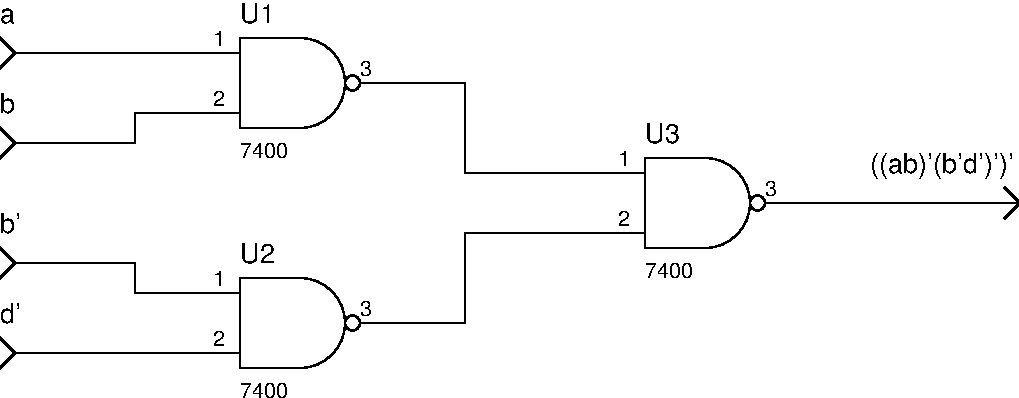
\includegraphics[scale=0.5]{nand-01}
\caption{Circuit definition of NAND (Equation \ref{eq:nand}).}
\label{fig:nand}
\end{figure}

Again using the simplified logic function (Equation \ref{eq:simp}) this
can be converted to use only NOR (not or) operations.
Equation \ref{eq:nor} shows this result.
An implementation of this function using gates is shown in Figure \ref{fig:nor}.

\begin{align}
f(a,b,c,d) &= a b + b'd' &\mbox{(original equation)} \notag \\
	&= (a b)'' + (b'd')'' \notag \\
	&= \left[ (a' + b')' + (b + d)' \right]'' &\mbox{(NOR form)} \label{eq:nor}
\end{align}

\begin{figure}[!hbtp]
\center
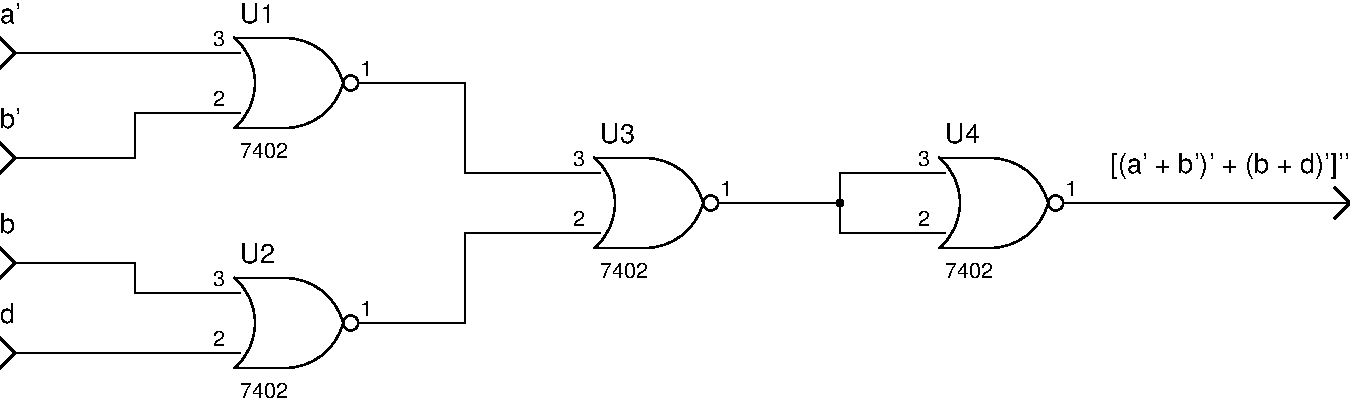
\includegraphics[scale=0.5]{nor-01}
\caption{Circuit definition of NOR (Equation \ref{eq:nor}).}
\label{fig:nor}
\end{figure}

\clearpage

\section{Observations}

The output of each logic function implemented in hardware
(Figure \ref{fig:nand}, Figure \ref{fig:nor}) agreed with the expected values
of the truth table (Figure \ref{fig:tt}).

\section{Conclusion}

This lab was a success in showing that a simplified function,
implemented in hardware using only NAND's or only NOR's,
will produce an equivalent function.

% flush all the figures
%\clearpage

%\pagebreak
%\renewcommand*{\refname}{\vspace{-8mm}}
%\section{References}
%%\bibliographystyle{plain}
%%\bibliographystyle{mslapa}
%\bibliographystyle{ieeetr}
%\bibliography{../references}

% Appendix (if needed)

\end{document}

% vim:foldmethod=marker
